\begin{abstract}
This working research dossier documents a completed 40-by-40 simulation of coordinated wildfire inspection by three drones. Independent implementations of DQN, REINFORCE and synchronous A2C were compared with Greedy, sweep, random and masked random baselines on untouched evaluation scenarios. The nine trained policies maintained zero drone losses under a common rule-based feasibility filter, but did not demonstrate better inspection quality than the Greedy baseline or consistent learning beyond masked random.
\end{abstract}
\begin{IEEEkeywords}reinforcement learning, wildfire inspection, drone fleet, DQN, REINFORCE, A2C\end{IEEEkeywords}
\section{Project description and critical review}
\subsection{Problem}
A central controller directs three battery-constrained drones to maintain fresh inspection coverage over changing wildfire hazards. This is a fully observed simulated inspection problem rather than a hidden-fire discovery task. Fuel, terrain susceptibility, burning state, inspection age, wind, battery, drone positions and charger ownership affect the decision process. A single charger and simultaneous motion introduce scheduling and collision constraints.
\subsection{Markov decision process}
The finite-horizon MDP has observations containing five complete grid maps of shape $(5,40,40)$, three drone records of shape $(3,4)$ and 12 global features. Neural policy inputs additionally derive four position channels from observed state. An action is a simultaneous triple of one of five commands: stay, north, south, west or east. Thus the centralized discrete action set contains $5^3=125$ joint commands. Transitions resolve moves and collisions, allocate one charging opportunity, update energy and losses, refresh nearby inspections, compute reward and evolve fire and wind using seeded random draws. The main horizon is 300 steps, battery capacity 160, recharge rate 8, inspection radius 2 and deadline 30.
The site weight is $w_i=p_i(1+2b_i+f_i)$ for static priority $p_i$, burning indicator $b_i$ and fire-front indicator $f_i$. Weighted freshness is $F_t=\sum_i w_i\max(0,1-a_i/d)/\sum_i w_i$, where $a_i$ is inspection age and $d=30$. Reward adds inspection gain and subtracts overdue, normalized energy, blocked moves and drone losses. A total fleet failure additionally incurs a remaining-horizon penalty. The simulation parameters are illustrative rather than physically calibrated.
\subsection{Implemented agents}
DQN predicts 125 joint-action values and uses replay, a target network, TD updates and epsilon-greedy exploration. REINFORCE computes full-episode discounted reward-to-go and uses a learned Monte Carlo value baseline without TD bootstrap. A2C combines a policy head with a state-value head, computes bootstrapped 32-step targets and trains synchronously. The source implementations are in \texttt{src/wild\_drone/learning.py} and \texttt{masked\_learning.py}; environment and baselines are implemented separately. The 40-by-40 study uses state-dependent feasible-action filtering for learned policies and masked random. The mask itself supplies safety rules and must not be attributed to neural learning.
\subsection{Training and evaluation}
The frozen study trained DQN, REINFORCE and A2C for 300 episodes per independent seed (0, 1, 2), nine fits and 810,000 interactions in total. Training worlds were 0--299. Final untouched scenarios were 22000--22019, yielding 180 RL missions and 80 baseline missions. All methods used discount $\gamma=0.99$ and gradient clipping at 0.5. DQN used learning rate $10^{-4}$, a 2,000-item replay and batch size 32; REINFORCE used $10^{-3}$; A2C used $10^{-4}$ and 32-step rollouts. No final-test checkpoint search, warm start or additional coordination shaping occurred.
\begin{table}[!t]\centering\caption{Frozen 40-by-40 evaluation means}\scriptsize
\begin{tabular}{lrrr}\toprule
Policy & Freshness & Return & Losses\\\midrule
DQN & .08438 & -24.79 & 0\\
REINFORCE & .06901 & -25.81 & 0\\
A2C & .08435 & -24.83 & 0\\
Greedy & .22077 & -16.10 & 0\\
Sweep & .06486 & -26.07 & 0\\
Random & .05956 & -42.87 & 3\\
Masked random & .08379 & -25.46 & 0\\\bottomrule
\end{tabular}\end{table}
\begin{figure}[!t]\centering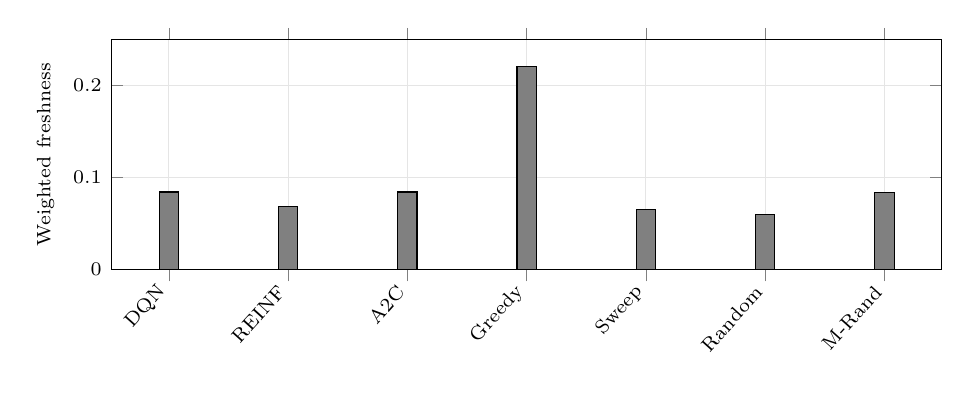
\begin{tikzpicture}
\begin{axis}[ybar,width=\columnwidth,height=4.5cm,bar width=7pt,ymin=0,ymax=.25,ylabel={Weighted freshness},symbolic x coords={DQN,REINF,A2C,Greedy,Sweep,Random,M-Rand},xtick=data,x tick label style={rotate=48,anchor=east,font=\scriptsize},ylabel style={font=\scriptsize},yticklabel style={font=\scriptsize},grid=major,major grid style={gray!20},enlarge x limits=.08]
\addplot[fill=black!50,draw=black] coordinates {(DQN,.08438) (REINF,.06901) (A2C,.08435) (Greedy,.22077) (Sweep,.06486) (Random,.05956) (M-Rand,.08379)};
\end{axis}\end{tikzpicture}

\caption{Priority-weighted inspection freshness on final 40-by-40 scenarios.}\end{figure}
\begin{figure}[!t]\centering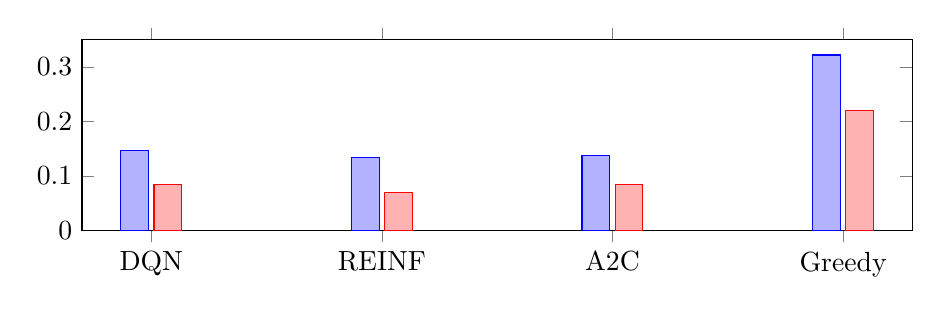
\begin{tikzpicture}
\begin{axis}[ybar,width=\columnwidth,height=4cm,ymin=0,ymax=0.35,symbolic x coords={DQN,REINF,A2C,Greedy},xtick=data]
\addplot coordinates {(DQN,.14585) (REINF,.13343) (A2C,.13694) (Greedy,.32203)};
\addplot coordinates {(DQN,.08438) (REINF,.06901) (A2C,.08435) (Greedy,.22077)};
\end{axis}
\end{tikzpicture}

\caption{Historical 20-by-20 and frozen 40-by-40 figures are descriptive, not a controlled scaling intervention.}\end{figure}
\subsection{Critical evaluation}
DQN exceeds masked random freshness by only 0.000589; A2C by 0.000553, while REINFORCE is worse. Greedy is far better than any learned controller on inspection freshness and reward. The all-seed learned-contribution and Greedy-capability criteria fail for every method. All 180 masked RL missions preserve three drones, but masked random also records no losses; unmasked random loses all three drones in all 20 missions. Therefore safe survival largely reflects feasibility constraints, not demonstrated autonomous coordination. Learned-model uncertainty is calculated across three fitted-seed means, each averaging 20 worlds; repeated worlds are not independent network fits. Sample SD of freshness across fit means is .00254 for DQN, .00730 for REINFORCE and .01163 for A2C.
An independent replay audit verified 75,911 evaluation steps, selected actions, state hashes, masks and rewards. This supports reproducibility within the simulator, not real-world flight validation. Historical results show poor action ranking, collision repetition and weak long-horizon charger coordination. The 20-by-20 experiments used different configurations and code revisions, so apparent cross-grid differences cannot be interpreted as the causal effect of grid size.
\section{Improvements linked to measured limitations}
\subsection{Structured cooperative credit assignment}
The 125-way central action head complicates attributing outcomes to individual drones. An independently evaluated factorised or counterfactual coordination model could estimate contributions from each drone while preserving fleet-level safety. Measure fresh-world timeliness, return scheduling and action interactions against masked random and Greedy; compare fixed interaction budgets. QMIX and COMA provide relevant research foundations.
\subsection{Potential-based inspection urgency}
Long-horizon timeliness remains poor under the current reward. A potential based on overdue priority and feasible travel-to-inspection opportunities could supply a denser learning signal while retaining the original evaluation objective. Use a difference of the form $\gamma\Phi(s')-\Phi(s)$, then test whether policy quality improves under matched data, while verifying the assumptions of policy invariance.
\subsection{Learner-state coverage}
Supervised ranking diagnostics fit observed labels but deteriorated in autonomous rollouts. Study data collection from states actually visited by the learner, including charger queues and critical battery margins, and compare with a uniformly sampled control set. Evaluate autonomous 300-step return, freshness and failure; training label accuracy alone is insufficient.
\section{Distinct extensions beyond present limitations}
\subsection{Belief-based inspection under uncertain sensing}
The current system observes true fire conditions directly. Expand to a POMDP with delayed, imperfect detections, learned belief maps and metrics such as detection latency and calibration. This changes the research objective from maintaining known-state inspection freshness to decisions under uncertainty.
\subsection{Decentralised communication-constrained fleets}
Replace the single central policy with local controllers and bounded message delays or packet loss. Study task completion against communication volume and coordination latency. This extends mission structure rather than simply retuning existing parameters.
\subsection{Calibrated heterogeneous operational environments}
Introduce geographically referenced scenarios, variable aircraft capabilities, richer weather, terrain and no-fly constraints, together with held-out environment regimes. Assess robust operation and risk-aware resource allocation; do not claim the current cellular fire model has validated physical accuracy.
\section{Individual contributions}
The group must independently identify authors for each notebook, code and report section, and agree on member-level percentages totaling 100\%. Contributor names and percentages are deliberately not invented in this research dossier.
\section*{References for independent verification}
\begin{thebibliography}{99}
\bibitem{study} Wild Drone Appeared, ``Frozen 40x40 RL main study,'' project repository, 2026.
\bibitem{dqn} V. Mnih et al., ``Human-level control through deep reinforcement learning,'' Nature, vol. 518, 2015.
\bibitem{reinforce} R. J. Williams, ``Simple statistical gradient-following algorithms,'' Machine Learning, 1992.
\bibitem{a2c} V. Mnih et al., ``Asynchronous methods for deep reinforcement learning,'' ICML, 2016.
\bibitem{qmix} T. Rashid et al., ``QMIX: Monotonic value function factorisation,'' ICML, 2018.
\bibitem{coma} J. N. Foerster et al., ``Counterfactual multi-agent policy gradients,'' AAAI, 2018.
\bibitem{shaping} A. Y. Ng et al., ``Policy invariance under reward transformations,'' ICML, 1999.
\bibitem{uav} K. D. Julian and M. J. Kochenderfer, ``Distributed wildfire surveillance with autonomous aircraft,'' J. Guidance Control Dynamics, 2019.
\bibitem{fire} A. Viseras et al., ``Wildfire front monitoring with multiple UAVs using deep Q-learning,'' IEEE Access, 2021.
\bibitem{cql} A. Kumar et al., ``Conservative Q-Learning for offline reinforcement learning,'' NeurIPS, 2020.
\bibitem{comm} J. N. Foerster et al., ``Learning to communicate with deep multi-agent reinforcement learning,'' NeurIPS, 2016.
\end{thebibliography}

\appendices
\section{Verification pointers}
The authoritative implementation is \texttt{Wildfire\_Drone\_Fleet.ipynb}, \texttt{src/wild\_drone/environment.py}, \texttt{learning.py}, \texttt{masked\_learning.py}, \texttt{configs/rl-main-frozen.json} and \texttt{docs/experiments/rl-main-2026-10-11/summary.csv}. The official specification requires no more than eight A4 two-column pages excluding references and appendices and at least six academic works supporting improvements and extensions. This study material does not replace an independently prepared submission.
